\documentclass{standalone}
\usepackage{tikz}
\usetikzlibrary{patterns, positioning}
\usepackage[sfdefault]{ClearSans} %% option 'sfdefault' activates Clear Sans as the default text font
\usepackage[T1]{fontenc}

\begin{document}
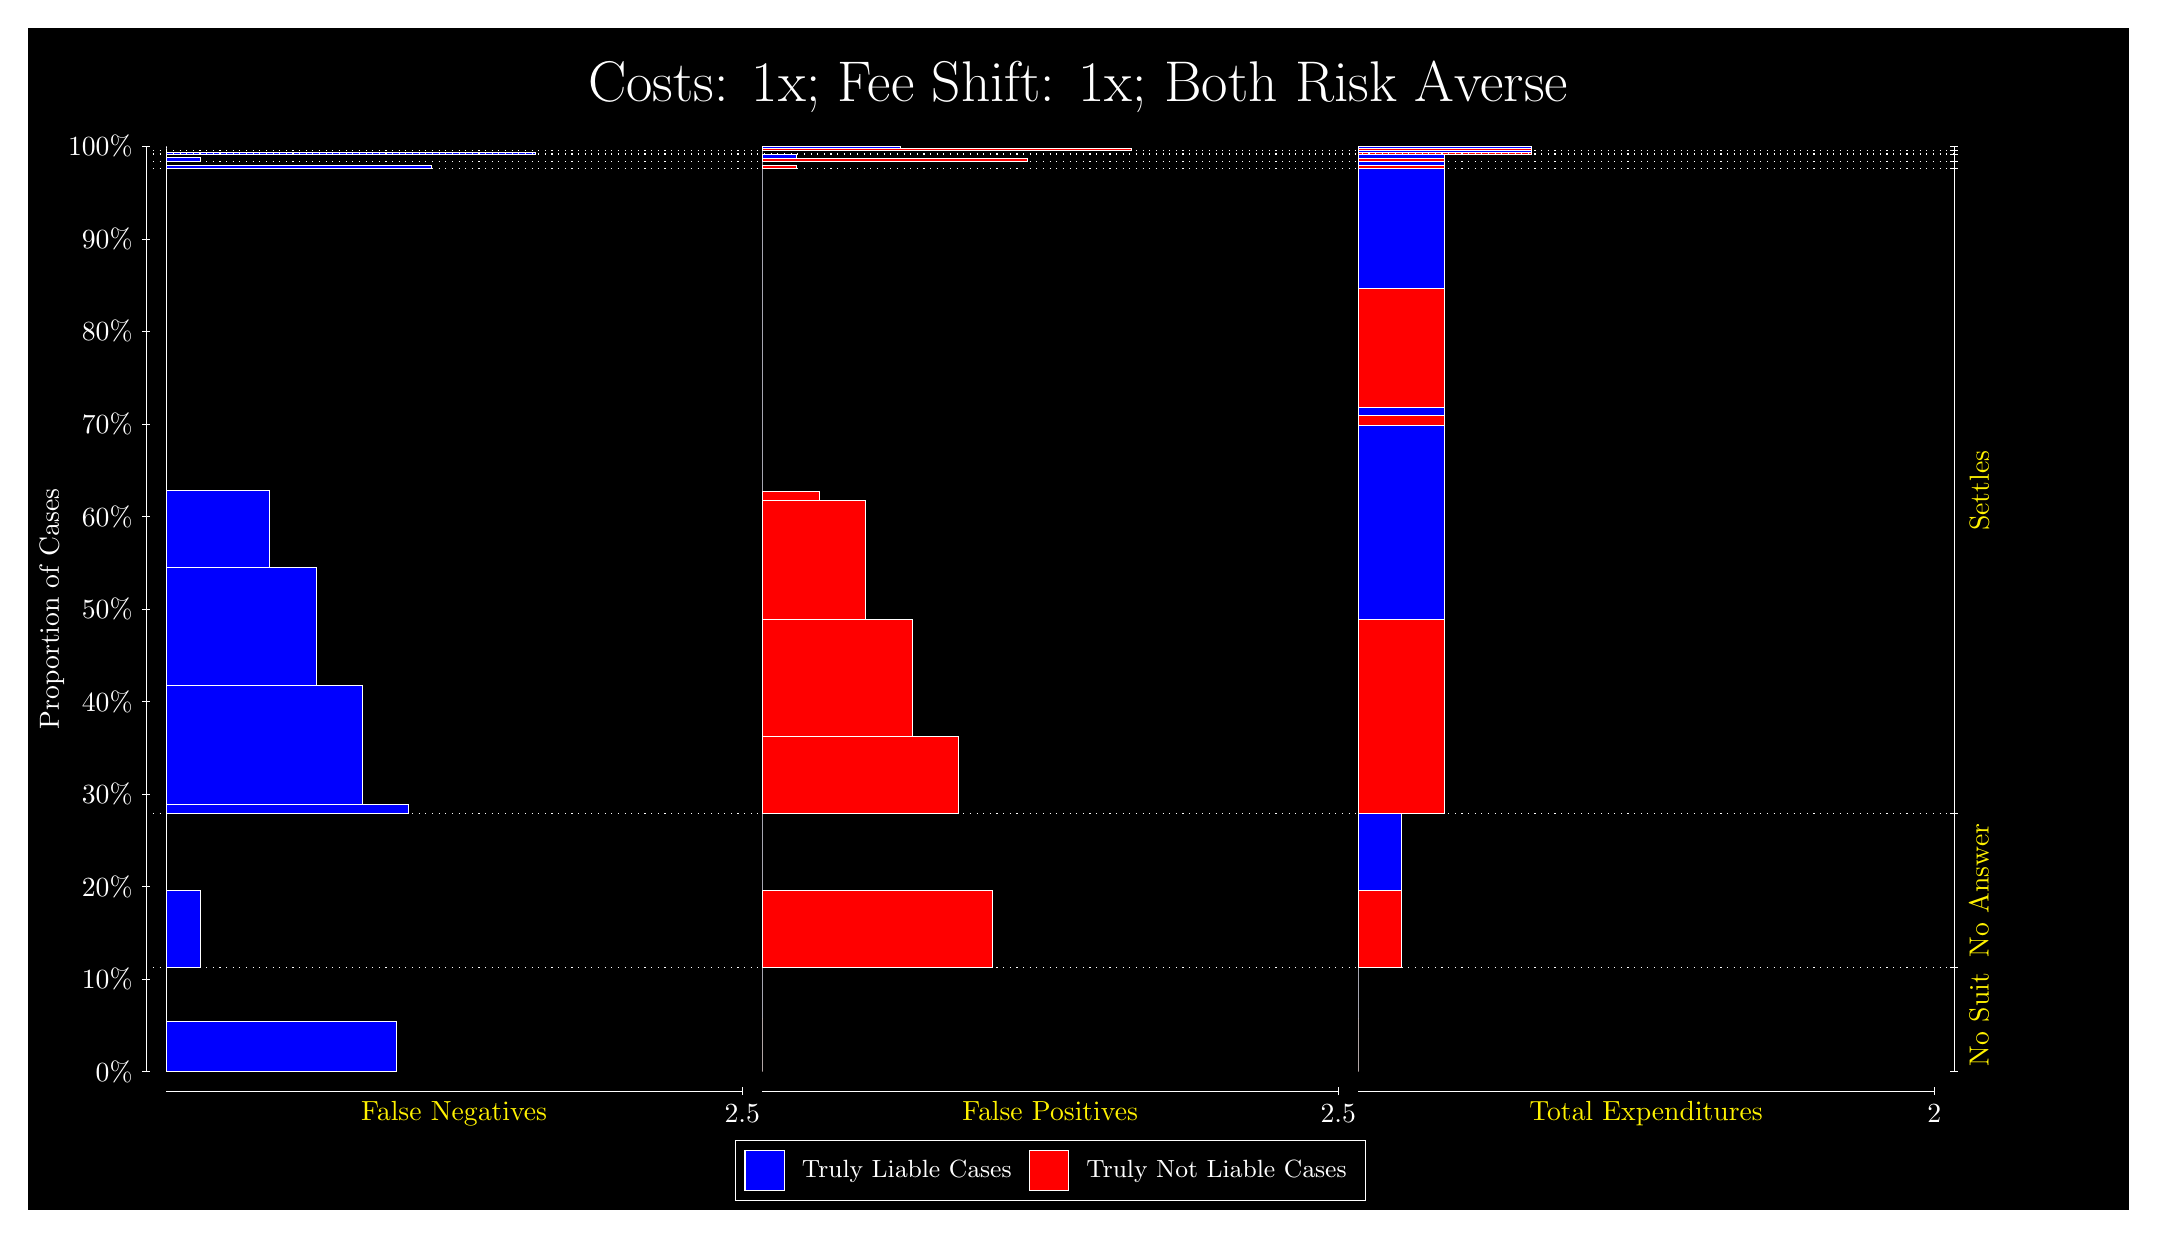
\begin{tikzpicture}
\draw[fill=black] (0,0) rectangle (26.667,15);
\draw[text=white] (0,13.5) rectangle (26.667,15) node[midway] {\huge Costs: 1x; Fee Shift: 1x; Both Risk Averse};
\draw[white, very thin] (1.5,1.75) -- (1.5,13.5);
\node[rotate=90, text=white, anchor=center] at (0.3, 7.625) {Proportion of Cases};
\draw[white, very thin] (1.45,1.75) -- (1.55,1.75);
\node[text=white, anchor=east] at (1.45, 1.75) {0\%};
\draw[white, very thin] (1.45,2.925) -- (1.55,2.925);
\node[text=white, anchor=east] at (1.45, 2.925) {10\%};
\draw[white, very thin] (1.45,4.1) -- (1.55,4.1);
\node[text=white, anchor=east] at (1.45, 4.1) {20\%};
\draw[white, very thin] (1.45,5.275) -- (1.55,5.275);
\node[text=white, anchor=east] at (1.45, 5.275) {30\%};
\draw[white, very thin] (1.45,6.45) -- (1.55,6.45);
\node[text=white, anchor=east] at (1.45, 6.45) {40\%};
\draw[white, very thin] (1.45,7.625) -- (1.55,7.625);
\node[text=white, anchor=east] at (1.45, 7.625) {50\%};
\draw[white, very thin] (1.45,8.8) -- (1.55,8.8);
\node[text=white, anchor=east] at (1.45, 8.8) {60\%};
\draw[white, very thin] (1.45,9.975) -- (1.55,9.975);
\node[text=white, anchor=east] at (1.45, 9.975) {70\%};
\draw[white, very thin] (1.45,11.15) -- (1.55,11.15);
\node[text=white, anchor=east] at (1.45, 11.15) {80\%};
\draw[white, very thin] (1.45,12.325) -- (1.55,12.325);
\node[text=white, anchor=east] at (1.45, 12.325) {90\%};
\draw[white, very thin] (1.45,13.5) -- (1.55,13.5);
\node[text=white, anchor=east] at (1.45, 13.5) {100\%};

\draw[white, very thin] (24.457,1.75) -- (24.457,13.5);
\draw[white, very thin] (24.407,1.75) -- (24.507,1.75);
\node[anchor=west] at (24.407, 1.75) {};
\draw[white, very thin] (24.407,3.0704) -- (24.507,3.0704);
\node[anchor=west] at (24.407, 3.0704) {};
\draw[white, very thin] (24.407,5.0287) -- (24.507,5.0287);
\node[anchor=west] at (24.407, 5.0287) {};
\draw[white, very thin] (24.407,13.223) -- (24.507,13.223);
\node[anchor=west] at (24.407, 13.223) {};
\draw[white, very thin] (24.407,13.304) -- (24.507,13.304);
\node[anchor=west] at (24.407, 13.304) {};
\draw[white, very thin] (24.407,13.402) -- (24.507,13.402);
\node[anchor=west] at (24.407, 13.402) {};
\draw[white, very thin] (24.407,13.451) -- (24.507,13.451);
\node[anchor=west] at (24.407, 13.451) {};
\draw[white, very thin] (24.407,13.5) -- (24.507,13.5);
\node[anchor=west] at (24.407, 13.5) {};

\draw[white, very thin, fill=blue] (1.75,1.75) rectangle (4.6775,2.3926);
\draw[white, very thin, fill=red] (1.75,2.3926) rectangle (1.75,3.0704);
\draw[white, very thin, fill=blue] (1.75,3.0704) rectangle (2.1891,4.0495);
\draw[white, very thin, fill=red] (1.75,4.0495) rectangle (1.75,5.0287);
\draw[white, very thin, fill=blue] (1.75,5.0287) rectangle (4.8239,5.1381);
\draw[white, very thin, fill=blue] (1.75,5.1381) rectangle (4.2384,6.6595);
\draw[white, very thin, fill=blue] (1.75,6.6595) rectangle (3.6529,8.1509);
\draw[white, very thin, fill=blue] (1.75,8.1509) rectangle (3.0674,9.1301);
\draw[white, very thin, fill=red] (1.75,9.1301) rectangle (1.75,13.223);
\draw[white, very thin, fill=blue] (1.75,13.223) rectangle (5.1167,13.264);
\draw[white, very thin, fill=red] (1.75,13.264) rectangle (1.75,13.304);
\draw[white, very thin, fill=blue] (1.75,13.304) rectangle (2.1891,13.363);
\draw[white, very thin, fill=red] (1.75,13.363) rectangle (1.75,13.402);
\draw[white, very thin, fill=blue] (1.75,13.402) rectangle (6.4341,13.426);
\draw[white, very thin, fill=red] (1.75,13.426) rectangle (1.75,13.451);
\draw[white, very thin, fill=red] (1.75,13.451) rectangle (1.75,13.472);
\draw[white, very thin, fill=blue] (1.75,13.472) rectangle (1.75,13.5);
\draw[white, very thin, fill=red] (9.3189,1.75) rectangle (9.3189,2.4277);
\draw[white, very thin, fill=blue] (9.3189,2.4277) rectangle (9.3189,3.0704);
\draw[white, very thin, fill=red] (9.3189,3.0704) rectangle (12.246,4.0495);
\draw[white, very thin, fill=blue] (9.3189,4.0495) rectangle (9.3189,5.0287);
\draw[white, very thin, fill=red] (9.3189,5.0287) rectangle (11.807,6.0079);
\draw[white, very thin, fill=red] (9.3189,6.0079) rectangle (11.222,7.4926);
\draw[white, very thin, fill=red] (9.3189,7.4926) rectangle (10.636,9.0031);
\draw[white, very thin, fill=red] (9.3189,9.0031) rectangle (10.051,9.1217);
\draw[white, very thin, fill=blue] (9.3189,9.1217) rectangle (9.3189,13.223);
\draw[white, very thin, fill=red] (9.3189,13.223) rectangle (9.758,13.263);
\draw[white, very thin, fill=blue] (9.3189,13.263) rectangle (9.3189,13.304);
\draw[white, very thin, fill=red] (9.3189,13.304) rectangle (12.686,13.343);
\draw[white, very thin, fill=blue] (9.3189,13.343) rectangle (9.758,13.402);
\draw[white, very thin, fill=red] (9.3189,13.402) rectangle (9.3189,13.427);
\draw[white, very thin, fill=blue] (9.3189,13.427) rectangle (9.3189,13.451);
\draw[white, very thin, fill=red] (9.3189,13.451) rectangle (14.003,13.472);
\draw[white, very thin, fill=blue] (9.3189,13.472) rectangle (11.075,13.5);
\draw[white, very thin, fill=red] (16.888,1.75) rectangle (16.888,2.4277);
\draw[white, very thin, fill=blue] (16.888,2.4277) rectangle (16.888,3.0704);
\draw[white, very thin, fill=red] (16.888,3.0704) rectangle (17.437,4.0495);
\draw[white, very thin, fill=blue] (16.888,4.0495) rectangle (17.437,5.0287);
\draw[white, very thin, fill=red] (16.888,5.0287) rectangle (17.986,7.4926);
\draw[white, very thin, fill=blue] (16.888,7.4926) rectangle (17.986,9.9632);
\draw[white, very thin, fill=red] (16.888,9.9632) rectangle (17.986,10.082);
\draw[white, very thin, fill=blue] (16.888,10.082) rectangle (17.986,10.191);
\draw[white, very thin, fill=red] (16.888,10.191) rectangle (17.986,11.702);
\draw[white, very thin, fill=blue] (16.888,11.702) rectangle (17.986,13.223);
\draw[white, very thin, fill=red] (16.888,13.223) rectangle (17.986,13.263);
\draw[white, very thin, fill=blue] (16.888,13.263) rectangle (17.986,13.304);
\draw[white, very thin, fill=red] (16.888,13.304) rectangle (17.986,13.343);
\draw[white, very thin, fill=blue] (16.888,13.343) rectangle (17.986,13.402);
\draw[white, very thin, fill=red] (16.888,13.402) rectangle (19.083,13.427);
\draw[white, very thin, fill=blue] (16.888,13.427) rectangle (19.083,13.451);
\draw[white, very thin, fill=red] (16.888,13.451) rectangle (19.083,13.472);
\draw[white, very thin, fill=blue] (16.888,13.472) rectangle (19.083,13.5);
\draw[white, dotted] (1.5,3.0704) -- (24.457,3.0704);
\draw[white, dotted] (1.5,5.0287) -- (24.457,5.0287);
\draw[white, dotted] (1.5,13.223) -- (24.457,13.223);
\draw[white, dotted] (1.5,13.304) -- (24.457,13.304);
\draw[white, dotted] (1.5,13.402) -- (24.457,13.402);
\draw[white, dotted] (1.5,13.451) -- (24.457,13.451);
\draw[white, very thin] (1.75,1.5) -- (9.0689,1.5);
\node[text=yellow, anchor=north] at (5.4094, 1.5) {False Negatives};
\draw[white, very thin] (9.0689,1.45) -- (9.0689,1.55);
\node[text=white, anchor=north] at (9.0689, 1.45) {2.5};

\draw[white, very thin] (9.3189,1.5) -- (16.638,1.5);
\node[text=yellow, anchor=north] at (12.978, 1.5) {False Positives};
\draw[white, very thin] (16.638,1.45) -- (16.638,1.55);
\node[text=white, anchor=north] at (16.638, 1.45) {2.5};

\draw[white, very thin] (16.888,1.5) -- (24.207,1.5);
\node[text=yellow, anchor=north] at (20.547, 1.5) {Total Expenditures};
\draw[white, very thin] (24.207,1.45) -- (24.207,1.55);
\node[text=white, anchor=north] at (24.207, 1.45) {2};

\node[text=yellow, centered, rotate=90] at (24.777, 2.4102) {No Suit};
\node[text=yellow, centered, rotate=90] at (24.777, 4.0495) {No Answer};
\node[text=yellow, centered, rotate=90] at (24.777, 9.1259) {Settles};





\draw (12.978300999999998,1.5) node[draw=none] (baseCoordinate) {};
\begin{scope}[align=center]
        \matrix[scale=0.5, draw=white, below=0.5cm of baseCoordinate, nodes={draw}, column sep=0.1cm]{
            \node[rectangle, draw, minimum width=0.5cm, minimum height=0.5cm, fill=blue] {}; &
            \node[draw=none, font=\small, text=white] (B) {Truly Liable Cases}; &
            \node[rectangle, draw, minimum width=0.5cm, minimum height=0.5cm, fill=red] {}; &
            \node[draw=none, font=\small, text=white] (B) {Truly Not Liable Cases}; \\
            };
\end{scope}

\end{tikzpicture}
\end{document}